\documentclass[twocolumn, 12pt]{article}
\usepackage[a4paper]{geometry}
\usepackage{titling}
\usepackage{ragged2e}
\usepackage[small, raggedright, compact]{titlesec}
\usepackage{microtype}
\usepackage{moresize}
\usepackage[rgb, dvipsnames]{xcolor}
\usepackage{tikz}
%% Turing poster design
%% ====================
%%
%% Fonts
%% -----
%% Our corporate brand is Neue Haas Unica Pro, but we don't have a general
%% license to use it. Our corporate substitute font is Arial, perhaps because
%% Windows has Arial. But Helvetica is closer in design to Neue Haas Unica Pro,
%% and I don't think Arial is available on Linux by default.
\usepackage{helvet}
\renewcommand{\familydefault}{\sfdefault}
\renewcommand{\baselinestretch}{1.1}
%%
%% Layout
%% ------
%% The portrait Turing poster appears to use a 9 vertical x 21 horizontal
%% grid. The actual measurements in the PowerPoint don't quite match, but
%% presumably the gris is what was intended.
\newlength{\gridv}\setlength{\gridv}{0.11111111111111111\paperheight}
\newlength{\gridh}\setlength{\gridh}{0.04761904761904762\paperwidth}
\geometry{hmargin=\gridh, columnsep=\gridh, top=\gridv, bottom=\gridh}
%%
%%
%% Logo
%% ----
%%
\definecolor{turingblue}{Hsb}{211,1,1}
\pagestyle{empty}
%%
%% Title
%% -----
\setlength{\droptitle}{-2em}
\pretitle{\rule{15\gridh}{4.6pt}\medskip\setlength{\rightskip}{5\gridh}\par%
\RaggedRight\begingroup\Huge\bfseries}
\posttitle{\endgroup\par\vskip 2em}
\preauthor{\setlength{\rightskip}{5\gridh}\par\begingroup\raggedright\large}
\postauthor{\endgroup\par\vskip 1em}
\predate{\begingroup\raggedright\large}
\postdate{\endgroup\par\vskip 2em}
%%
%% Section headers
%% ---------------
\titleformat{\section}{\titlerule[3.2pt]\bfseries\large}{\thesection}{1em}{}{}
\titlespacing*{\section}{0em}{*4}{*1}
%%
\RaggedRight{}
%%
%% =============================================================================
%% Actual content from here on down
%%
\usepackage{amsmath}
\usepackage{enumitem}
\usepackage{minted}
\title{Nocell: Programming prob\-ab\-il\-ist\-ic spreadsheets}
\author{James Geddes, Oliver Strickson, and Tom Counsell}
\date{}
\begin{document}
\maketitle
\thispagestyle{empty}
%%
%% Yes, you have to put the section header before the background image. Sorry. This is a problem: tikz
%% images take up space where they are "made", even if, like this one, they are moved somewhere
%% absolute. Not sure what to do about this as I don't understand tikz sufficiently well.
\section*{Overview}
%%
Spreadsheets are great! Everyone \textcolor{OliveGreen}{\bfseries understands} them, everyone
\textcolor{OliveGreen}{\bfseries uses} them.

Spreadsheets are terrible! No \textcolor{red}{\bfseries modularity}, no
\textcolor{red}{\bfseries abstraction}, no \textcolor{red}{\bfseries code re-use}, no
\textcolor{red}{\bfseries version control}. And no \textcolor{red}{\bfseries inference}.

Nocell is a programming language for writing probabilistic spreadsheets.


\section*{A classic example: How much is HSBC worth?}
\small
Under a discount rate $D$, the \emph{present value} of a stream of cashflows
$c_i$ in years $i=0,\dotsc,N-1$, followed by cashflows from year $N$ of $f$,
increasing annually by a rate $R$ is:
\[
\text{PV} = \sum_{i = 0}^{N-1} \frac{c_i}{{(1 + d)}^{i}}  +
\frac{1}{{(1+d)}^N} \frac{f}{d-r}.
\]

\subsection*{As a program...}
{\tiny
\inputminted{scheme}{dcf.nocell}
}

\subsection*{...which compiles to a spreadsheet}
\begin{center}
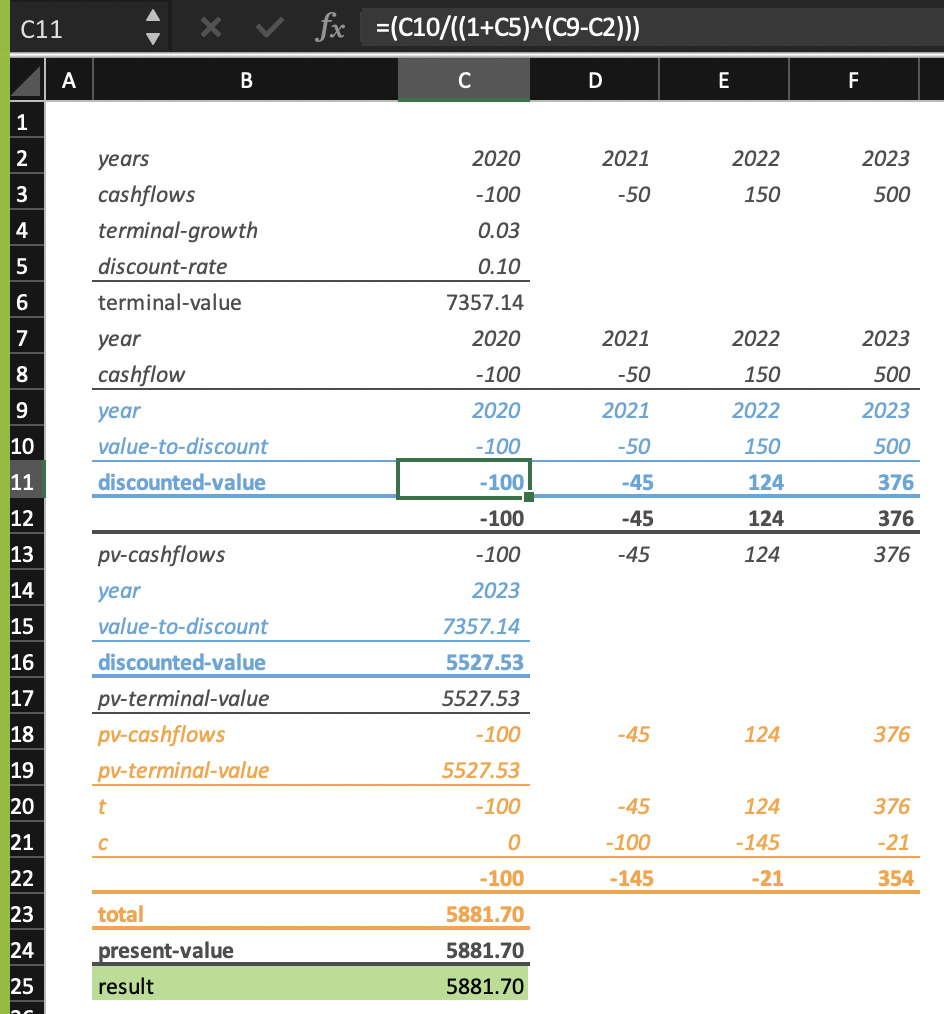
\includegraphics[width=0.75\columnwidth]{figs/ss.png}
\end{center}

\section*{How it works}
\begin{center}
\includegraphics[width=\columnwidth]{figs/languages.eps}
\end{center}
\begin{itemize}[itemsep=0.4ex]
\item ‘nocell’ is a probabilistic programming language with bounded recursion.
\item ‘cell’ is a non--Turing-complete language for calculating with tabular
  data.
\item ‘grid’ is a model of a spreadsheet: a purely functional programming language with no loops.
\end{itemize}

\section*{Ongoing work}
\begin{itemize}[nosep]
\item Representation of distributions in spreadsheets
\item Design and layout
\item Recursion
\end{itemize}
  
\vfill
\section*{Contact}

James Geddes, \texttt{jgeddes@turing.ac.uk}.
\begin{tikzpicture}[remember picture,overlay]
\fill[fill=turingblue] (current page.north east) -- +(-17\gridh, 0) -- +(-2\gridh, -\gridv) -- +(0, -0.6\gridv) -- +(0,0);
\node [above] (image) at (current page.north east) [xshift=-2\gridh,yshift=-0.6\gridv] {
\includegraphics[height=0.4\gridv]{ATI_logo_white.eps}};
\end{tikzpicture}
\end{document}
